\documentclass[12pt]{article}
\usepackage[tmargin=1.5in]{geometry}
\usepackage{relsize}
\usepackage{babel}
\usepackage{listings}
\usepackage{amsmath}
\usepackage{amssymb}
\usepackage[table]{xcolor}
\usepackage[pdftex]{graphicx}
\usepackage{caption}
\usepackage{color}
\usepackage{xparse}

\setlength{\parindent}{0cm}  % Indentation prohibited by default
% \captionsetup[figure]{labelformat=empty}    % Remove figure labels

\newcommand{\cfbox}[2]{\fcolorbox{black}{#1}{#2}}

\definecolor{aquamarine}{RGB}{182.8, 255.0, 95}
\definecolor{greyblue}{RGB}{159, 159, 188}
\definecolor{mypurple}{RGB}{188, 98, 170}
\definecolor{bluegreen}{RGB}{6, 157, 152}
\definecolor{lapislazuli}{RGB}{82, 122, 157}
\definecolor{harvestgold}{RGB}{206, 134, 18}
\definecolor{yellowgreen}{RGB}{8, 217, 53}

\title{Aufgabenblatt 7: Circle}
\author{Gruppe: CaesarBaurMueller}
\date{\today}

\begin{document}
\maketitle

\begin{sloppypar}
    
\section*{Aufgabe 1: Circle}
\subsubsection*{Formel}
Die Formel für die Anzahl der Elemente, welche jeder Prozess bearbeiten muss:
\begin{equation}
    \begin{aligned}
        Elements\_for\_each\_Process = \frac{N}{nprocs}
    \end{aligned}
\end{equation}
Die Formel für die Anzahl der Prozesse, die ein Zusatzelement behandeln müssen:
\begin{equation}
    \begin{aligned}
        Processes\_with\_additional\_Element = N \mod nprocs
    \end{aligned}
\end{equation}

\subsubsection*{Visualisierung}

\begin{figure}[ht]
    \begin{minipage}[t]{0.3\textwidth}
        \begin{flushright}
            Start \\ \vspace*{1.4pt}
        \end{flushright}
        \begin{flushright}
            Iteration 0 \\ \vspace*{1.4pt}
        \end{flushright}
        \begin{flushright}
            Iteration 1 \\ \vspace*{1.4pt}
        \end{flushright}
        \begin{flushright}
            Iteration 2 \\ \vspace*{1.4pt}
        \end{flushright}
        \begin{flushright}
            Iteration 3 \\
        \end{flushright}
    \end{minipage}
    \hspace*{0.08\textwidth}
    \begin{minipage}[t]{0.6\textwidth}
        $
        \cfbox{greyblue}{9}
        \cfbox{greyblue}{23}
        \cfbox{greyblue}{1}
        \cfbox{mypurple}{4}
        \cfbox{mypurple}{1}
        \cfbox{mypurple}{14}
        \cfbox{bluegreen}{18}
        \cfbox{bluegreen}{1}
        \cfbox{bluegreen}{6}
        \cfbox{yellowgreen}{24}
        \cfbox{yellowgreen}{7}
        \cfbox{harvestgold}{4}
        \cfbox{harvestgold}{17}
        $ \\ \\
        $
        \cfbox{harvestgold}{4}
        \cfbox{harvestgold}{17}
        \cfbox{greyblue}{9}
        \cfbox{greyblue}{23}
        \cfbox{greyblue}{1}
        \cfbox{mypurple}{4}
        \cfbox{mypurple}{1}
        \cfbox{mypurple}{14}
        \cfbox{bluegreen}{18}
        \cfbox{bluegreen}{1}
        \cfbox{bluegreen}{6}
        \cfbox{yellowgreen}{24}
        \cfbox{yellowgreen}{7}
        $ \\ \\
        $
        \cfbox{yellowgreen}{24}
        \cfbox{yellowgreen}{7}
        \cfbox{harvestgold}{4}
        \cfbox{harvestgold}{17}
        \cfbox{greyblue}{9}
        \cfbox{greyblue}{23}
        \cfbox{greyblue}{1}
        \cfbox{mypurple}{4}
        \cfbox{mypurple}{1}
        \cfbox{mypurple}{14}
        \cfbox{bluegreen}{18}
        \cfbox{bluegreen}{1}
        \cfbox{bluegreen}{6}
        $ \\ \\
        $
        \cfbox{bluegreen}{18}
        \cfbox{bluegreen}{1}
        \cfbox{bluegreen}{6}
        \cfbox{yellowgreen}{24}
        \cfbox{yellowgreen}{7}
        \cfbox{harvestgold}{4}
        \cfbox{harvestgold}{17}
        \cfbox{greyblue}{9}
        \cfbox{greyblue}{23}
        \cfbox{greyblue}{1}
        \cfbox{mypurple}{4}
        \cfbox{mypurple}{1}
        \cfbox{mypurple}{14}
        $ \\ \\
        $
        \cfbox{mypurple}{4}
        \cfbox{mypurple}{1}
        \cfbox{mypurple}{14}
        \cfbox{bluegreen}{18}
        \cfbox{bluegreen}{1}
        \cfbox{bluegreen}{6}
        \cfbox{yellowgreen}{24}
        \cfbox{yellowgreen}{7}
        \cfbox{harvestgold}{4}
        \cfbox{harvestgold}{17}
        \cfbox{greyblue}{9}
        \cfbox{greyblue}{23}
        \cfbox{greyblue}{1}
        $
    \end{minipage}
\end{figure}

\newpage

\section{Aufgabe 2: Vampir}

\subsubsection*{Richtung der Kommunikation}
Die Richtung der Kommunikation ist in der graphischen Darstellung von Links nach Rechts zu lesen. Somit ist der linke Punkt in Vampir der Sender und der Rechte Punkt der Empfänger. Hierbei ist allerdings zu beachten, dass es keine global synchronisierte Zeit gibt und es daher etwas verzerrt wirken kann.

\subsubsection*{Kommunikationsmatrix}
\begin{figure}[ht]
    \centering
    \caption{Kommunikationsmatrix}
    \begin{minipage}[t]{\textwidth}
        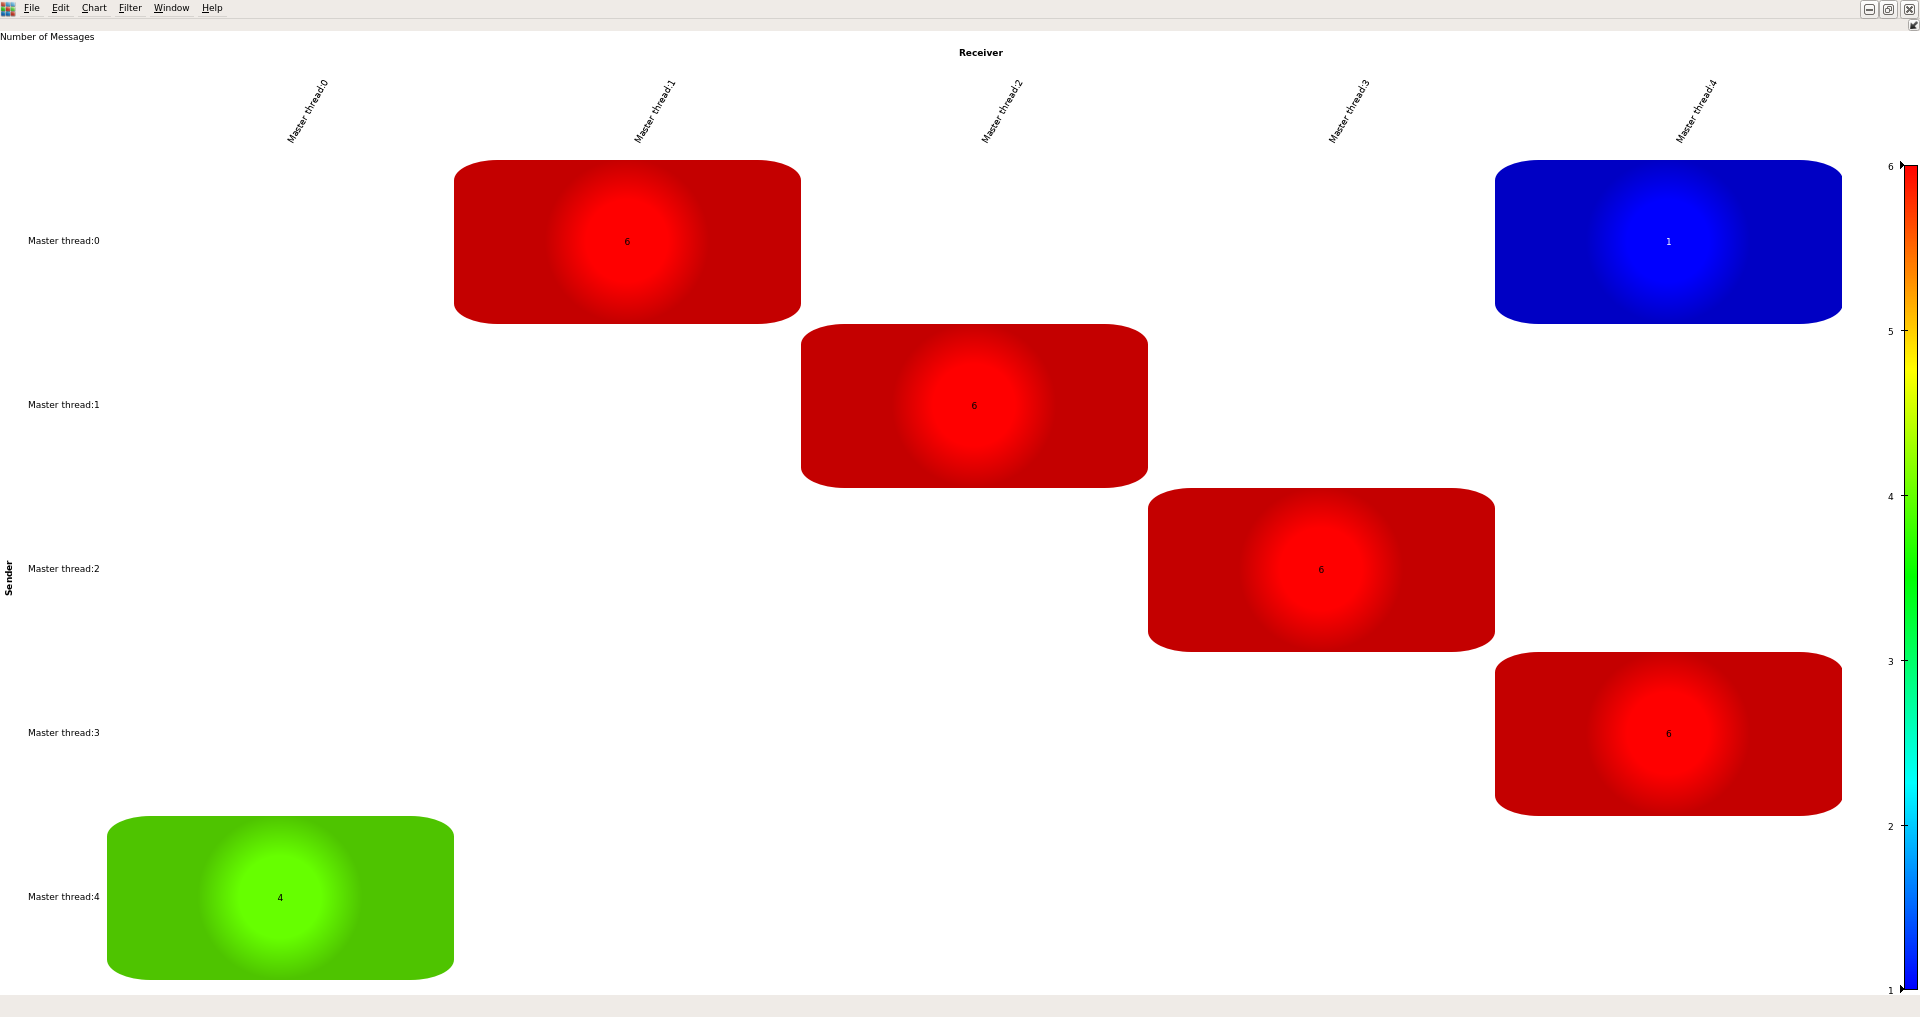
\includegraphics[width=\textwidth]{res/Communication_Matrix.png}
    \end{minipage}
\end{figure}

\subsubsection*{Programmphasen}
\begin{figure}[ht]
    \caption*{Graphische Darstellung der Kommunikation}
    \begin{minipage}[t]{1.2\textwidth}
        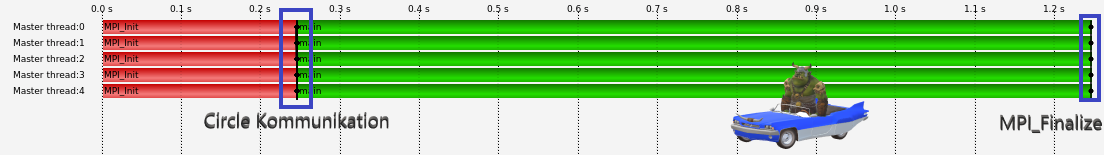
\includegraphics[width=0.8\textwidth]{res/Master_Timeline_edited.png}
    \end{minipage}
\end{figure}

\subsubsection*{Dauer der INIT Phase}
Die \verb|MPI Init| Phase hat durchschnittlich etwa \textit{0.245} Sekunden gedauert.
\begin{figure}[ht]
    \centering
    \caption*{Dauer der \textit{MPI\_INIT} Phase}
    \begin{minipage}[t]{0.3\textwidth}
        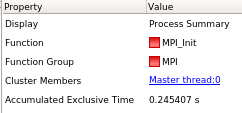
\includegraphics[width=\textwidth]{res/init-phase-p0.PNG}
    \end{minipage}
    \begin{minipage}[t]{0.12\textwidth}
        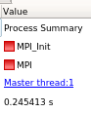
\includegraphics[width=\textwidth]{res/init-phase-p1.PNG}
    \end{minipage}
    \begin{minipage}[t]{0.12\textwidth}
        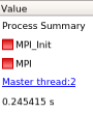
\includegraphics[width=\textwidth]{res/init-phase-p2.PNG}
    \end{minipage}
    \begin{minipage}[t]{0.12\textwidth}
        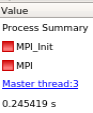
\includegraphics[width=\textwidth]{res/init-phase-p3.PNG}
    \end{minipage}
    \begin{minipage}[t]{0.12\textwidth}
        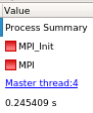
\includegraphics[width=\textwidth]{res/init-phase-p4.PNG}
    \end{minipage}
\end{figure}


\section{Aufgabe 3: Parallelisierung mit MPI}
\subsubsection*{Formel}
Unsere Formel ist die Folgende:
\begin{equation}
    lines = (interlines * 8) + 9
\end{equation}
Sie ist die Summe der Zeilen, die durch die Interlines entstehen $(interlines * 8)$, 
plus die Zeilen, die für die Darstellung der Elemente am Ende existieren $(9)$. Die $-2$ aus der Berechnung auf den vorigen Blättern benötigen wir hier nicht mehr, da wir die Randzeilen in die Berechnung mit aufnehmen (wenn auch nur als Hilfswerte). Die Prozesse $P_0$ und $P_{last}$ müssen sie also in ihren Speicher aufnehmen. \\

Für die Interlines gilt somit $i \in N_0$. \\
Für die Prozesse können wir bei Programmstart festlegen, welche Anzahl wir für die Berechnung
verwenden wollen. Somit ist $t$ für die Berechnung von $i$ irrelevant. Es kann berechnet 
werden, wie viele Zeilen jeder Prozess berechnen muss, um eine effiziente Bearbeitung 
zu gewährleisten. Die Formel hierfür lautet:
\begin{equation}
    lines per Process = \frac{lines}{n\_procs}
\end{equation}
Es gilt $n\_procs \in \mathbb{N}$. Wenn $n\_procs < 1$ gewählt wird, wird dies vom Programm nicht zugelassen. Wenn die Lines durch die Prozesse nicht aufgehen, wird der Rest auf die ersten Prozesse aufgeteilt, dass ein Teil der Prozesse eine Line mehr als der Rest zu bearbeiten hat. \\
Sollten weniger Lines als Prozesse gewählt werden, wird der Rest der Prozesse nicht gestartet. \\
Es ergibt sich zusammengefasst die folgende Formel:
\begin{equation}
    lines\_per\_process = \frac{(interlines * 8) + 9}{n\_procs}
\end{equation}

\subsubsection*{Schleifenköpfe}
Hierfür definieren wir folgende Variable: \\

\verb|int lines_per_process = ((interlines * 8) + 9) / n_procs;| \\

sowie eine Variable \verb|int offset|, welche den Offset für die \verb|starting_row| darstellt (da einige Prozesse mehr Zeilen haben können als andere). Daraus ergeben sich: \\

\verb|int starting_row = offset + (lines_per_process * rank) + 1;|
\verb|int ending_row = starting_row + lines_per_process + 1;|

\begin{center}
    \vspace*{0.5em}
    \begin{tabular*}{\textwidth}[ht]{r|l}
        Rang 0 & \verb|for(int i = starting_row (1); i < ending_row (6); i++)| \\
        Rang 2 & \verb|for(int i = starting_row (11); i < ending_row (16); i++)| \\
        Rang 4 & \verb|for(int i = starting_row (20); i < ending_row (24); i++)| \\
    \end{tabular*}
\end{center}

\newpage
\subsubsection*{Visualisierung}
\begin{figure}[h]
    \centering
    \begin{minipage}[t]{0.13\textwidth}
        \begin{flushright}
            \vspace*{2.5em}
            $P_0$ \\ \vspace*{1.7em}
            $com. P_0P_1$ \\ \vspace*{2.5em}
            $P_1$ \\ \vspace*{2.1em}
            $com. P_1P_2$ \\ \vspace*{2.5em}
            $P_2$ \\ \vspace*{2.1em}
            $com. P_2P_3$ \\ \vspace*{2.5em}
            $P_3$ \\ \vspace*{2.1em}
            $com. P_3P_4$ \\ \vspace*{1.7em}
            $P_4$ \\
        \end{flushright}
    \end{minipage}
    \hspace*{0.05\textwidth}
    \begin{minipage}[t]{0.8\textwidth}
        $
        \cfbox{yellowgreen}{1}
        \cfbox{yellowgreen}{1}
        \cfbox{yellowgreen}{1}
        \cfbox{yellowgreen}{1}
        \cfbox{yellowgreen}{1}
        \cfbox{yellowgreen}{1}
        \cfbox{yellowgreen}{1}
        \cfbox{yellowgreen}{1}
        \cfbox{yellowgreen}{1}
        \cfbox{yellowgreen}{1}
        \cfbox{yellowgreen}{1}
        \cfbox{yellowgreen}{1}
        \cfbox{yellowgreen}{1}
        \cfbox{yellowgreen}{1}
        \cfbox{yellowgreen}{1}
        \cfbox{yellowgreen}{1}
        \cfbox{yellowgreen}{1}
        \cfbox{yellowgreen}{1}
        \cfbox{yellowgreen}{1}
        \cfbox{yellowgreen}{1}
        \cfbox{yellowgreen}{1}
        \cfbox{yellowgreen}{1}
        \cfbox{yellowgreen}{1}
        \cfbox{yellowgreen}{1}
        \cfbox{yellowgreen}{1}
        $ \\
        $
        \cfbox{yellowgreen}{1}
        \cfbox{bluegreen}{0}
        \cfbox{bluegreen}{0}
        \cfbox{bluegreen}{0}
        \cfbox{bluegreen}{0}
        \cfbox{bluegreen}{0}
        \cfbox{bluegreen}{0}
        \cfbox{bluegreen}{0}
        \cfbox{bluegreen}{0}
        \cfbox{bluegreen}{0}
        \cfbox{bluegreen}{0}
        \cfbox{bluegreen}{0}
        \cfbox{bluegreen}{0}
        \cfbox{bluegreen}{0}
        \cfbox{bluegreen}{0}
        \cfbox{bluegreen}{0}
        \cfbox{bluegreen}{0}
        \cfbox{bluegreen}{0}
        \cfbox{bluegreen}{0}
        \cfbox{bluegreen}{0}
        \cfbox{bluegreen}{0}
        \cfbox{bluegreen}{0}
        \cfbox{bluegreen}{0}
        \cfbox{bluegreen}{0}
        \cfbox{yellowgreen}{1}
        $ \\
        $
        \cfbox{yellowgreen}{1}
        \cfbox{bluegreen}{0}
        \cfbox{bluegreen}{0}
        \cfbox{bluegreen}{0}
        \cfbox{bluegreen}{0}
        \cfbox{bluegreen}{0}
        \cfbox{bluegreen}{0}
        \cfbox{bluegreen}{0}
        \cfbox{bluegreen}{0}
        \cfbox{bluegreen}{0}
        \cfbox{bluegreen}{0}
        \cfbox{bluegreen}{0}
        \cfbox{bluegreen}{0}
        \cfbox{bluegreen}{0}
        \cfbox{bluegreen}{0}
        \cfbox{bluegreen}{0}
        \cfbox{bluegreen}{0}
        \cfbox{bluegreen}{0}
        \cfbox{bluegreen}{0}
        \cfbox{bluegreen}{0}
        \cfbox{bluegreen}{0}
        \cfbox{bluegreen}{0}
        \cfbox{bluegreen}{0}
        \cfbox{bluegreen}{0}
        \cfbox{yellowgreen}{1}
        $ \\
        $
        \cfbox{yellowgreen}{1}
        \cfbox{bluegreen}{0}
        \cfbox{bluegreen}{0}
        \cfbox{bluegreen}{0}
        \cfbox{bluegreen}{0}
        \cfbox{bluegreen}{0}
        \cfbox{bluegreen}{0}
        \cfbox{bluegreen}{0}
        \cfbox{bluegreen}{0}
        \cfbox{bluegreen}{0}
        \cfbox{bluegreen}{0}
        \cfbox{bluegreen}{0}
        \cfbox{bluegreen}{0}
        \cfbox{bluegreen}{0}
        \cfbox{bluegreen}{0}
        \cfbox{bluegreen}{0}
        \cfbox{bluegreen}{0}
        \cfbox{bluegreen}{0}
        \cfbox{bluegreen}{0}
        \cfbox{bluegreen}{0}
        \cfbox{bluegreen}{0}
        \cfbox{bluegreen}{0}
        \cfbox{bluegreen}{0}
        \cfbox{bluegreen}{0}
        \cfbox{yellowgreen}{1}
        $ \\
        $
        \cfbox{yellowgreen}{1}
        \cfbox{bluegreen}{↓}
        \cfbox{bluegreen}{↓}
        \cfbox{bluegreen}{↓}
        \cfbox{bluegreen}{↓}
        \cfbox{bluegreen}{↓}
        \cfbox{bluegreen}{↓}
        \cfbox{bluegreen}{↓}
        \cfbox{bluegreen}{↓}
        \cfbox{bluegreen}{↓}
        \cfbox{bluegreen}{↓}
        \cfbox{bluegreen}{↓}
        \cfbox{bluegreen}{↓}
        \cfbox{bluegreen}{↓}
        \cfbox{bluegreen}{↓}
        \cfbox{bluegreen}{↓}
        \cfbox{bluegreen}{↓}
        \cfbox{bluegreen}{↓}
        \cfbox{bluegreen}{↓}
        \cfbox{bluegreen}{↓}
        \cfbox{bluegreen}{↓}
        \cfbox{bluegreen}{↓}
        \cfbox{bluegreen}{↓}
        \cfbox{bluegreen}{↓}
        \cfbox{yellowgreen}{1}
        $ \\
        $
        \cfbox{yellowgreen}{1}
        \cfbox{mypurple}{↑}
        \cfbox{mypurple}{↑}
        \cfbox{mypurple}{↑}
        \cfbox{mypurple}{↑}
        \cfbox{mypurple}{↑}
        \cfbox{mypurple}{↑}
        \cfbox{mypurple}{↑}
        \cfbox{mypurple}{↑}
        \cfbox{mypurple}{↑}
        \cfbox{mypurple}{↑}
        \cfbox{mypurple}{↑}
        \cfbox{mypurple}{↑}
        \cfbox{mypurple}{↑}
        \cfbox{mypurple}{↑}
        \cfbox{mypurple}{↑}
        \cfbox{mypurple}{↑}
        \cfbox{mypurple}{↑}
        \cfbox{mypurple}{↑}
        \cfbox{mypurple}{↑}
        \cfbox{mypurple}{↑}
        \cfbox{mypurple}{↑}
        \cfbox{mypurple}{↑}
        \cfbox{mypurple}{↑}
        \cfbox{yellowgreen}{1}
        $ \\
        $
        \cfbox{yellowgreen}{1}
        \cfbox{mypurple}{0}
        \cfbox{mypurple}{0}
        \cfbox{mypurple}{0}
        \cfbox{mypurple}{0}
        \cfbox{mypurple}{0}
        \cfbox{mypurple}{0}
        \cfbox{mypurple}{0}
        \cfbox{mypurple}{0}
        \cfbox{mypurple}{0}
        \cfbox{mypurple}{0}
        \cfbox{mypurple}{0}
        \cfbox{mypurple}{0}
        \cfbox{mypurple}{0}
        \cfbox{mypurple}{0}
        \cfbox{mypurple}{0}
        \cfbox{mypurple}{0}
        \cfbox{mypurple}{0}
        \cfbox{mypurple}{0}
        \cfbox{mypurple}{0}
        \cfbox{mypurple}{0}
        \cfbox{mypurple}{0}
        \cfbox{mypurple}{0}
        \cfbox{mypurple}{0}
        \cfbox{yellowgreen}{1}
        $ \\
        $
        \cfbox{yellowgreen}{1}
        \cfbox{mypurple}{0}
        \cfbox{mypurple}{0}
        \cfbox{mypurple}{0}
        \cfbox{mypurple}{0}
        \cfbox{mypurple}{0}
        \cfbox{mypurple}{0}
        \cfbox{mypurple}{0}
        \cfbox{mypurple}{0}
        \cfbox{mypurple}{0}
        \cfbox{mypurple}{0}
        \cfbox{mypurple}{0}
        \cfbox{mypurple}{0}
        \cfbox{mypurple}{0}
        \cfbox{mypurple}{0}
        \cfbox{mypurple}{0}
        \cfbox{mypurple}{0}
        \cfbox{mypurple}{0}
        \cfbox{mypurple}{0}
        \cfbox{mypurple}{0}
        \cfbox{mypurple}{0}
        \cfbox{mypurple}{0}
        \cfbox{mypurple}{0}
        \cfbox{mypurple}{0}
        \cfbox{yellowgreen}{1}
        $ \\
        $
        \cfbox{yellowgreen}{1}
        \cfbox{mypurple}{0}
        \cfbox{mypurple}{0}
        \cfbox{mypurple}{0}
        \cfbox{mypurple}{0}
        \cfbox{mypurple}{0}
        \cfbox{mypurple}{0}
        \cfbox{mypurple}{0}
        \cfbox{mypurple}{0}
        \cfbox{mypurple}{0}
        \cfbox{mypurple}{0}
        \cfbox{mypurple}{0}
        \cfbox{mypurple}{0}
        \cfbox{mypurple}{0}
        \cfbox{mypurple}{0}
        \cfbox{mypurple}{0}
        \cfbox{mypurple}{0}
        \cfbox{mypurple}{0}
        \cfbox{mypurple}{0}
        \cfbox{mypurple}{0}
        \cfbox{mypurple}{0}
        \cfbox{mypurple}{0}
        \cfbox{mypurple}{0}
        \cfbox{mypurple}{0}
        \cfbox{yellowgreen}{1}
        $ \\
        $
        \cfbox{yellowgreen}{1}
        \cfbox{mypurple}{↓}
        \cfbox{mypurple}{↓}
        \cfbox{mypurple}{↓}
        \cfbox{mypurple}{↓}
        \cfbox{mypurple}{↓}
        \cfbox{mypurple}{↓}
        \cfbox{mypurple}{↓}
        \cfbox{mypurple}{↓}
        \cfbox{mypurple}{↓}
        \cfbox{mypurple}{↓}
        \cfbox{mypurple}{↓}
        \cfbox{mypurple}{↓}
        \cfbox{mypurple}{↓}
        \cfbox{mypurple}{↓}
        \cfbox{mypurple}{↓}
        \cfbox{mypurple}{↓}
        \cfbox{mypurple}{↓}
        \cfbox{mypurple}{↓}
        \cfbox{mypurple}{↓}
        \cfbox{mypurple}{↓}
        \cfbox{mypurple}{↓}
        \cfbox{mypurple}{↓}
        \cfbox{mypurple}{↓}
        \cfbox{yellowgreen}{1}
        $ \\
        $
        \cfbox{yellowgreen}{1}
        \cfbox{greyblue}{↑}
        \cfbox{greyblue}{↑}
        \cfbox{greyblue}{↑}
        \cfbox{greyblue}{↑}
        \cfbox{greyblue}{↑}
        \cfbox{greyblue}{↑}
        \cfbox{greyblue}{↑}
        \cfbox{greyblue}{↑}
        \cfbox{greyblue}{↑}
        \cfbox{greyblue}{↑}
        \cfbox{greyblue}{↑}
        \cfbox{greyblue}{↑}
        \cfbox{greyblue}{↑}
        \cfbox{greyblue}{↑}
        \cfbox{greyblue}{↑}
        \cfbox{greyblue}{↑}
        \cfbox{greyblue}{↑}
        \cfbox{greyblue}{↑}
        \cfbox{greyblue}{↑}
        \cfbox{greyblue}{↑}
        \cfbox{greyblue}{↑}
        \cfbox{greyblue}{↑}
        \cfbox{greyblue}{↑}
        \cfbox{yellowgreen}{1}
        $ \\
        $
        \cfbox{yellowgreen}{1}
        \cfbox{greyblue}{0}
        \cfbox{greyblue}{0}
        \cfbox{greyblue}{0}
        \cfbox{greyblue}{0}
        \cfbox{greyblue}{0}
        \cfbox{greyblue}{0}
        \cfbox{greyblue}{0}
        \cfbox{greyblue}{0}
        \cfbox{greyblue}{0}
        \cfbox{greyblue}{0}
        \cfbox{greyblue}{0}
        \cfbox{greyblue}{0}
        \cfbox{greyblue}{0}
        \cfbox{greyblue}{0}
        \cfbox{greyblue}{0}
        \cfbox{greyblue}{0}
        \cfbox{greyblue}{0}
        \cfbox{greyblue}{0}
        \cfbox{greyblue}{0}
        \cfbox{greyblue}{0}
        \cfbox{greyblue}{0}
        \cfbox{greyblue}{0}
        \cfbox{greyblue}{0}
        \cfbox{yellowgreen}{1}
        $ \\
        $
        \cfbox{yellowgreen}{1}
        \cfbox{greyblue}{0}
        \cfbox{greyblue}{0}
        \cfbox{greyblue}{0}
        \cfbox{greyblue}{0}
        \cfbox{greyblue}{0}
        \cfbox{greyblue}{0}
        \cfbox{greyblue}{0}
        \cfbox{greyblue}{0}
        \cfbox{greyblue}{0}
        \cfbox{greyblue}{0}
        \cfbox{greyblue}{0}
        \cfbox{greyblue}{0}
        \cfbox{greyblue}{0}
        \cfbox{greyblue}{0}
        \cfbox{greyblue}{0}
        \cfbox{greyblue}{0}
        \cfbox{greyblue}{0}
        \cfbox{greyblue}{0}
        \cfbox{greyblue}{0}
        \cfbox{greyblue}{0}
        \cfbox{greyblue}{0}
        \cfbox{greyblue}{0}
        \cfbox{greyblue}{0}
        \cfbox{yellowgreen}{1}
        $ \\
        $
        \cfbox{yellowgreen}{1}
        \cfbox{greyblue}{0}
        \cfbox{greyblue}{0}
        \cfbox{greyblue}{0}
        \cfbox{greyblue}{0}
        \cfbox{greyblue}{0}
        \cfbox{greyblue}{0}
        \cfbox{greyblue}{0}
        \cfbox{greyblue}{0}
        \cfbox{greyblue}{0}
        \cfbox{greyblue}{0}
        \cfbox{greyblue}{0}
        \cfbox{greyblue}{0}
        \cfbox{greyblue}{0}
        \cfbox{greyblue}{0}
        \cfbox{greyblue}{0}
        \cfbox{greyblue}{0}
        \cfbox{greyblue}{0}
        \cfbox{greyblue}{0}
        \cfbox{greyblue}{0}
        \cfbox{greyblue}{0}
        \cfbox{greyblue}{0}
        \cfbox{greyblue}{0}
        \cfbox{greyblue}{0}
        \cfbox{yellowgreen}{1}
        $ \\
        $
        \cfbox{yellowgreen}{1}
        \cfbox{greyblue}{↓}
        \cfbox{greyblue}{↓}
        \cfbox{greyblue}{↓}
        \cfbox{greyblue}{↓}
        \cfbox{greyblue}{↓}
        \cfbox{greyblue}{↓}
        \cfbox{greyblue}{↓}
        \cfbox{greyblue}{↓}
        \cfbox{greyblue}{↓}
        \cfbox{greyblue}{↓}
        \cfbox{greyblue}{↓}
        \cfbox{greyblue}{↓}
        \cfbox{greyblue}{↓}
        \cfbox{greyblue}{↓}
        \cfbox{greyblue}{↓}
        \cfbox{greyblue}{↓}
        \cfbox{greyblue}{↓}
        \cfbox{greyblue}{↓}
        \cfbox{greyblue}{↓}
        \cfbox{greyblue}{↓}
        \cfbox{greyblue}{↓}
        \cfbox{greyblue}{↓}
        \cfbox{greyblue}{↓}
        \cfbox{yellowgreen}{1}
        $ \\
        $
        \cfbox{yellowgreen}{1}
        \cfbox{lapislazuli}{↑}
        \cfbox{lapislazuli}{↑}
        \cfbox{lapislazuli}{↑}
        \cfbox{lapislazuli}{↑}
        \cfbox{lapislazuli}{↑}
        \cfbox{lapislazuli}{↑}
        \cfbox{lapislazuli}{↑}
        \cfbox{lapislazuli}{↑}
        \cfbox{lapislazuli}{↑}
        \cfbox{lapislazuli}{↑}
        \cfbox{lapislazuli}{↑}
        \cfbox{lapislazuli}{↑}
        \cfbox{lapislazuli}{↑}
        \cfbox{lapislazuli}{↑}
        \cfbox{lapislazuli}{↑}
        \cfbox{lapislazuli}{↑}
        \cfbox{lapislazuli}{↑}
        \cfbox{lapislazuli}{↑}
        \cfbox{lapislazuli}{↑}
        \cfbox{lapislazuli}{↑}
        \cfbox{lapislazuli}{↑}
        \cfbox{lapislazuli}{↑}
        \cfbox{lapislazuli}{↑}
        \cfbox{yellowgreen}{1}
        $\\
        $
        \cfbox{yellowgreen}{1}
        \cfbox{lapislazuli}{0}
        \cfbox{lapislazuli}{0}
        \cfbox{lapislazuli}{0}
        \cfbox{lapislazuli}{0}
        \cfbox{lapislazuli}{0}
        \cfbox{lapislazuli}{0}
        \cfbox{lapislazuli}{0}
        \cfbox{lapislazuli}{0}
        \cfbox{lapislazuli}{0}
        \cfbox{lapislazuli}{0}
        \cfbox{lapislazuli}{0}
        \cfbox{lapislazuli}{0}
        \cfbox{lapislazuli}{0}
        \cfbox{lapislazuli}{0}
        \cfbox{lapislazuli}{0}
        \cfbox{lapislazuli}{0}
        \cfbox{lapislazuli}{0}
        \cfbox{lapislazuli}{0}
        \cfbox{lapislazuli}{0}
        \cfbox{lapislazuli}{0}
        \cfbox{lapislazuli}{0}
        \cfbox{lapislazuli}{0}
        \cfbox{lapislazuli}{0}
        \cfbox{yellowgreen}{1}
        $ \\
        $
        \cfbox{yellowgreen}{1}
        \cfbox{lapislazuli}{0}
        \cfbox{lapislazuli}{0}
        \cfbox{lapislazuli}{0}
        \cfbox{lapislazuli}{0}
        \cfbox{lapislazuli}{0}
        \cfbox{lapislazuli}{0}
        \cfbox{lapislazuli}{0}
        \cfbox{lapislazuli}{0}
        \cfbox{lapislazuli}{0}
        \cfbox{lapislazuli}{0}
        \cfbox{lapislazuli}{0}
        \cfbox{lapislazuli}{0}
        \cfbox{lapislazuli}{0}
        \cfbox{lapislazuli}{0}
        \cfbox{lapislazuli}{0}
        \cfbox{lapislazuli}{0}
        \cfbox{lapislazuli}{0}
        \cfbox{lapislazuli}{0}
        \cfbox{lapislazuli}{0}
        \cfbox{lapislazuli}{0}
        \cfbox{lapislazuli}{0}
        \cfbox{lapislazuli}{0}
        \cfbox{lapislazuli}{0}
        \cfbox{yellowgreen}{1}
        $\\
        $
        \cfbox{yellowgreen}{1}
        \cfbox{lapislazuli}{0}
        \cfbox{lapislazuli}{0}
        \cfbox{lapislazuli}{0}
        \cfbox{lapislazuli}{0}
        \cfbox{lapislazuli}{0}
        \cfbox{lapislazuli}{0}
        \cfbox{lapislazuli}{0}
        \cfbox{lapislazuli}{0}
        \cfbox{lapislazuli}{0}
        \cfbox{lapislazuli}{0}
        \cfbox{lapislazuli}{0}
        \cfbox{lapislazuli}{0}
        \cfbox{lapislazuli}{0}
        \cfbox{lapislazuli}{0}
        \cfbox{lapislazuli}{0}
        \cfbox{lapislazuli}{0}
        \cfbox{lapislazuli}{0}
        \cfbox{lapislazuli}{0}
        \cfbox{lapislazuli}{0}
        \cfbox{lapislazuli}{0}
        \cfbox{lapislazuli}{0}
        \cfbox{lapislazuli}{0}
        \cfbox{lapislazuli}{0}
        \cfbox{yellowgreen}{1}
        $\\
        $
        \cfbox{yellowgreen}{1}
        \cfbox{lapislazuli}{↓}
        \cfbox{lapislazuli}{↓}
        \cfbox{lapislazuli}{↓}
        \cfbox{lapislazuli}{↓}
        \cfbox{lapislazuli}{↓}
        \cfbox{lapislazuli}{↓}
        \cfbox{lapislazuli}{↓}
        \cfbox{lapislazuli}{↓}
        \cfbox{lapislazuli}{↓}
        \cfbox{lapislazuli}{↓}
        \cfbox{lapislazuli}{↓}
        \cfbox{lapislazuli}{↓}
        \cfbox{lapislazuli}{↓}
        \cfbox{lapislazuli}{↓}
        \cfbox{lapislazuli}{↓}
        \cfbox{lapislazuli}{↓}
        \cfbox{lapislazuli}{↓}
        \cfbox{lapislazuli}{↓}
        \cfbox{lapislazuli}{↓}
        \cfbox{lapislazuli}{↓}
        \cfbox{lapislazuli}{↓}
        \cfbox{lapislazuli}{↓}
        \cfbox{lapislazuli}{↓}
        \cfbox{yellowgreen}{1}
        $ \\
        $
        \cfbox{yellowgreen}{1}
        \cfbox{harvestgold}{↑}
        \cfbox{harvestgold}{↑}
        \cfbox{harvestgold}{↑}
        \cfbox{harvestgold}{↑}
        \cfbox{harvestgold}{↑}
        \cfbox{harvestgold}{↑}
        \cfbox{harvestgold}{↑}
        \cfbox{harvestgold}{↑}
        \cfbox{harvestgold}{↑}
        \cfbox{harvestgold}{↑}
        \cfbox{harvestgold}{↑}
        \cfbox{harvestgold}{↑}
        \cfbox{harvestgold}{↑}
        \cfbox{harvestgold}{↑}
        \cfbox{harvestgold}{↑}
        \cfbox{harvestgold}{↑}
        \cfbox{harvestgold}{↑}
        \cfbox{harvestgold}{↑}
        \cfbox{harvestgold}{↑}
        \cfbox{harvestgold}{↑}
        \cfbox{harvestgold}{↑}
        \cfbox{harvestgold}{↑}
        \cfbox{harvestgold}{↑}
        \cfbox{yellowgreen}{1}
        $ \\
        $
        \cfbox{yellowgreen}{1}
        \cfbox{harvestgold}{0}
        \cfbox{harvestgold}{0}
        \cfbox{harvestgold}{0}
        \cfbox{harvestgold}{0}
        \cfbox{harvestgold}{0}
        \cfbox{harvestgold}{0}
        \cfbox{harvestgold}{0}
        \cfbox{harvestgold}{0}
        \cfbox{harvestgold}{0}
        \cfbox{harvestgold}{0}
        \cfbox{harvestgold}{0}
        \cfbox{harvestgold}{0}
        \cfbox{harvestgold}{0}
        \cfbox{harvestgold}{0}
        \cfbox{harvestgold}{0}
        \cfbox{harvestgold}{0}
        \cfbox{harvestgold}{0}
        \cfbox{harvestgold}{0}
        \cfbox{harvestgold}{0}
        \cfbox{harvestgold}{0}
        \cfbox{harvestgold}{0}
        \cfbox{harvestgold}{0}
        \cfbox{harvestgold}{0}
        \cfbox{yellowgreen}{1}
        $ \\
        $
        \cfbox{yellowgreen}{1}
        \cfbox{harvestgold}{0}
        \cfbox{harvestgold}{0}
        \cfbox{harvestgold}{0}
        \cfbox{harvestgold}{0}
        \cfbox{harvestgold}{0}
        \cfbox{harvestgold}{0}
        \cfbox{harvestgold}{0}
        \cfbox{harvestgold}{0}
        \cfbox{harvestgold}{0}
        \cfbox{harvestgold}{0}
        \cfbox{harvestgold}{0}
        \cfbox{harvestgold}{0}
        \cfbox{harvestgold}{0}
        \cfbox{harvestgold}{0}
        \cfbox{harvestgold}{0}
        \cfbox{harvestgold}{0}
        \cfbox{harvestgold}{0}
        \cfbox{harvestgold}{0}
        \cfbox{harvestgold}{0}
        \cfbox{harvestgold}{0}
        \cfbox{harvestgold}{0}
        \cfbox{harvestgold}{0}
        \cfbox{harvestgold}{0}
        \cfbox{yellowgreen}{1}
        $ \\
        $
        \cfbox{yellowgreen}{1}
        \cfbox{harvestgold}{0}
        \cfbox{harvestgold}{0}
        \cfbox{harvestgold}{0}
        \cfbox{harvestgold}{0}
        \cfbox{harvestgold}{0}
        \cfbox{harvestgold}{0}
        \cfbox{harvestgold}{0}
        \cfbox{harvestgold}{0}
        \cfbox{harvestgold}{0}
        \cfbox{harvestgold}{0}
        \cfbox{harvestgold}{0}
        \cfbox{harvestgold}{0}
        \cfbox{harvestgold}{0}
        \cfbox{harvestgold}{0}
        \cfbox{harvestgold}{0}
        \cfbox{harvestgold}{0}
        \cfbox{harvestgold}{0}
        \cfbox{harvestgold}{0}
        \cfbox{harvestgold}{0}
        \cfbox{harvestgold}{0}
        \cfbox{harvestgold}{0}
        \cfbox{harvestgold}{0}
        \cfbox{harvestgold}{0}
        \cfbox{yellowgreen}{1}
        $ \\
        $
        \cfbox{yellowgreen}{1}
        \cfbox{yellowgreen}{1}
        \cfbox{yellowgreen}{1}
        \cfbox{yellowgreen}{1}
        \cfbox{yellowgreen}{1}
        \cfbox{yellowgreen}{1}
        \cfbox{yellowgreen}{1}
        \cfbox{yellowgreen}{1}
        \cfbox{yellowgreen}{1}
        \cfbox{yellowgreen}{1}
        \cfbox{yellowgreen}{1}
        \cfbox{yellowgreen}{1}
        \cfbox{yellowgreen}{1}
        \cfbox{yellowgreen}{1}
        \cfbox{yellowgreen}{1}
        \cfbox{yellowgreen}{1}
        \cfbox{yellowgreen}{1}
        \cfbox{yellowgreen}{1}
        \cfbox{yellowgreen}{1}
        \cfbox{yellowgreen}{1}
        \cfbox{yellowgreen}{1}
        \cfbox{yellowgreen}{1}
        \cfbox{yellowgreen}{1}
        \cfbox{yellowgreen}{1}
        \cfbox{yellowgreen}{1}
        $
    \end{minipage}
\end{figure}
Wie der Matrix zu entnehmen ist, kommunizieren immer nur die Nachbarprozesse miteinander.
Die Randelemente stehen jeweils dem Prozess zur Verfügung, der an diese Elemente anliegt.
In diesem Beispiel ($i=2$ und $n\_procs=5$) erhält jeder Prozess insgesamt fünf Zeilen. Dies schließt bei den Prozessen $P_0$ und $P_4$ die jeweilige Randzeile mit ein. Grund hierfür ist die möglichst gleichmäßige Aufteilung von Zeilen auf die Prozesse und dass die Randzeilen für die Berechnung der Matrix benötigt werden (siehe Stern).
Hätten wir einen Fall in dem $n\_procs - 1$ Zeilen bei der Aufteilung übrig bleiben (bspw. $i=2$ und $n\_procs=6$), so würde der erste Prozess $P_0$ ebenfalls eine Zeile mehr erhalten, zuzüglich zu der Randzeile.

\subsubsection*{Kommunikationsschemata}
\begin{figure}[ht]
    \centering
    \caption*{Abbruch nach Iterationen \\ Kollektiv: \texttt{Barrier}}
    \begin{minipage}[t]{0.99\textwidth}
        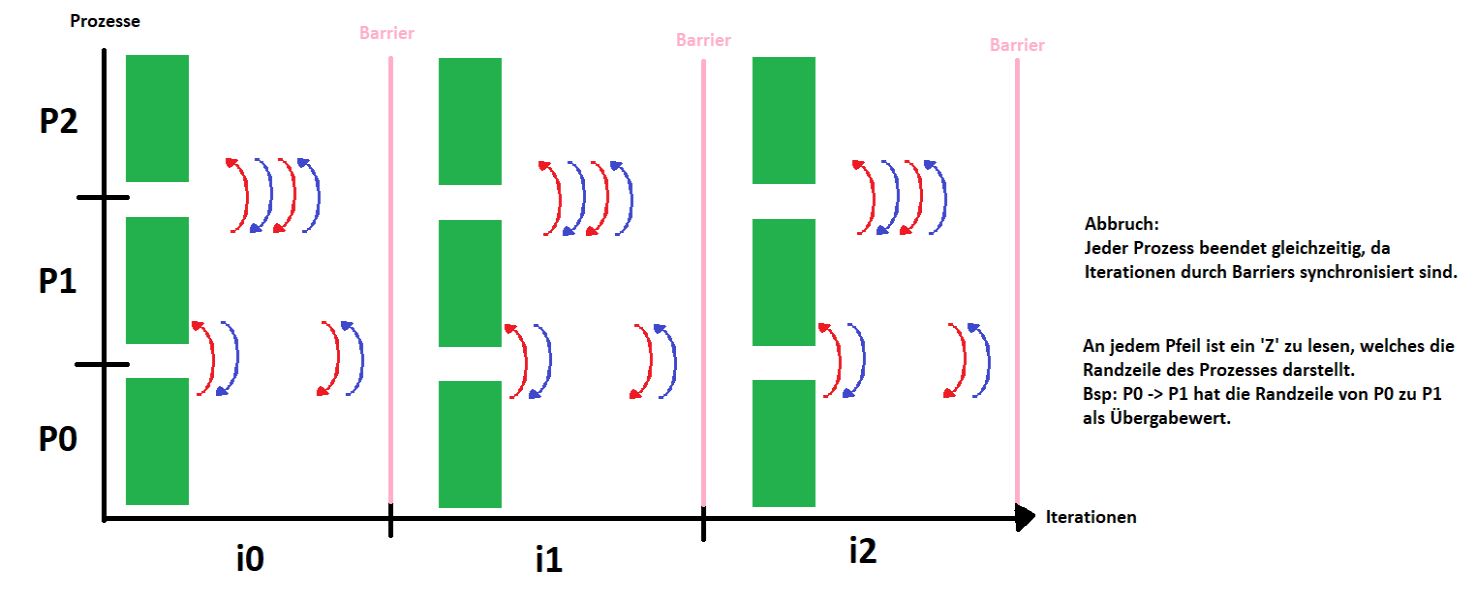
\includegraphics[width=\textwidth]{res/Kommunikation-Iterations.PNG}
    \end{minipage}
    \vspace*{2em}
    \caption*{Abbruch nach Genauigkeit \\ Kollektiv: \texttt{Gather}, \texttt{BCast}, \texttt{Barrier}}
    \begin{minipage}[t]{0.99\textwidth}
        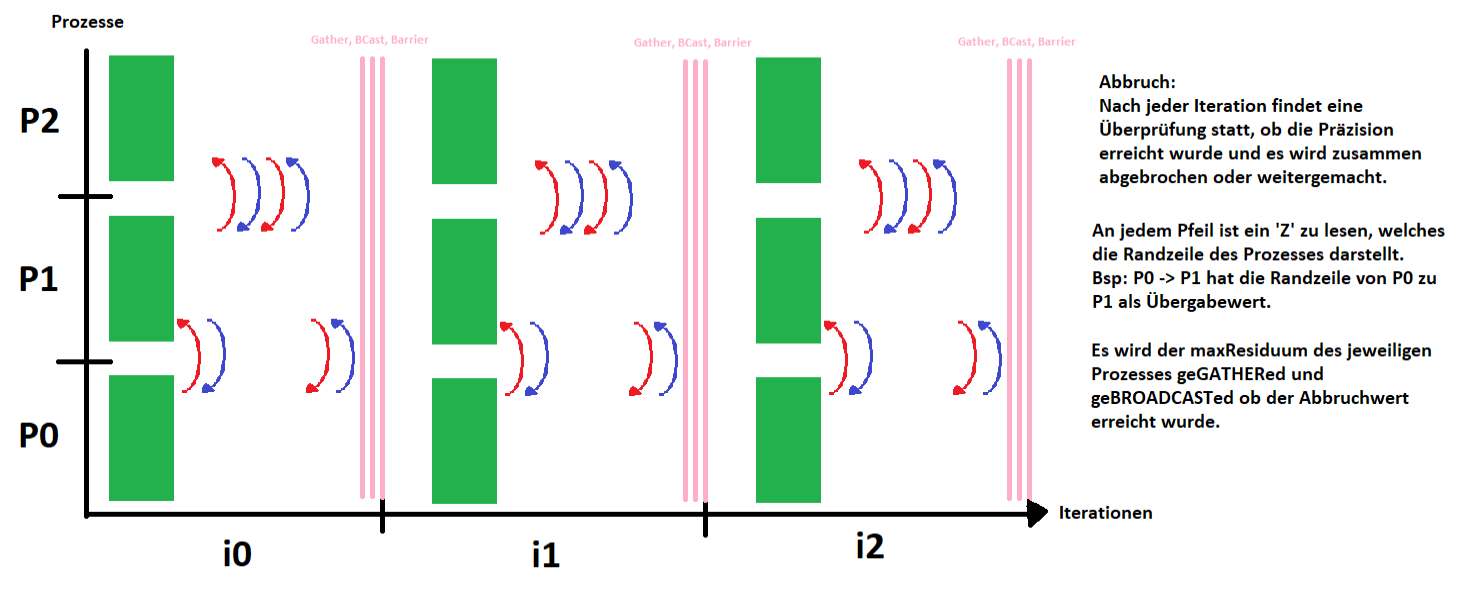
\includegraphics[width=\textwidth]{res/Kommunikation-Residuum.PNG}
    \end{minipage}
\end{figure}

Bei jeder Iteration werden die Randzeilen der Prozesse an die Nachbarprozesse gesendet. Dies birgt viel Aufwand. Schließlich gibt es nach jeder Iteration noch eine bzw. drei Kollektive Operationen, um die Prozesse zu synchronisieren. \\

\end{sloppypar}

\end{document}